%!TEX root = ../EmbSW2.tex
\section{Algorithmen}

\subsection{Beschreibungsmethoden}
\begin{itemize}
	\item Aktivitätsdiagramm $\rightarrow$ gute Variante!
	\item Konkrete Programmiersprache $\rightarrow$ gute Variante!
	\item Pseudocode
	\item Struktogramme $\rightarrow$ veraltet
	\item Programmablaufpläne $\rightarrow$ veraltet
\end{itemize}

\subsection{Formale Eigenschaften}
\subsubsection{Korrektheit}
    \begin{itemize}
	    \item Die Korrektheit eines Algorithmus kann formal bewiesen werden. Dies ist jedoch häufig mit enormem Aufwand verbunden und wird in der Praxis nur selten durchgeführt $\rightarrow$ In der Praxis wird die Korrektheit mit Tests verifiziert.
	    \item Nur \textbf{Anwesenheit von Fehlern} kann bewiesen werden, nicht deren Abwesenheit [E.Dijkstra]
    \end{itemize}
\subsubsection{Finitheit}
    \begin{itemize}
	    \item Der Algorithmus muss eindeutig mit einer endlichen Anzahl Schritten beschrieben werden können.
    \end{itemize}
\subsubsection{Bestimmtheit}
    \begin{itemize}
	    \item Der Algorithmus erzielt bei gleichen Vorbedingungen immer dasselbe Resultat (bei Algorithmen, die mit Zufallskomponenten arbeiten, trifft das nicht zu).
    \end{itemize}
\subsubsection{Determinismus}
    \begin{itemize}
	    \item Zu jedem Zeitpunkt ist der nächste Schritt des Algorithmus eindeutig bestimmt.
    \end{itemize}
\subsubsection{Effizienz}
    \begin{itemize}
	    \item Laufzeiteffizienz
	    \item Speicherplatzeffizienz
	    \item Verschiedene Betrachtungsweisen:
	    \begin{itemize}
	        \item Best Case: Optimistischer Fall
	        \item Average Case: Durchschnittlicher Fall
	        \item Worst case (üblich): Pessimistischer Fall
	    \end{itemize}
    \end{itemize}
\subsubsection{Optionale formale Eigenschaften}
    \begin{itemize}
	    \item Einfachheit
	    \item Verständlichkeit
    \end{itemize}


\subsection{Komplexitätstheorie}
\subsubsection{Hauptziele}
    \begin{itemize}
        \item Berechnungskomplexität: Zeitkomplexität als Anzahl der Rechenoperationen sowie Speicherplatzkomplexität
        \item Spezifikation der Probleme und Methode zur Klassifikation in "'praktisch lösbare"' und "'praktisch unlösbare"' Probleme
        \item Vergleiche der Effizienz (Berechnungsstärke) verschiedener Algorithmen (deterministischer, nichtdeterministischer und zufallsgesteuerter)
    \end{itemize}
\subsubsection{Zu betrachtende Operationen}
\begin{multicols}{2}
    \begin{itemize}
        \item Zuweisungen (Bewegung von Datensätzen)
        \item Vergleiche
        \item Rechenoperationen
        \item Unterprogrammaufrufe
        \item Verzweigungen
    \end{itemize}
		\vfill\null
		\columnbreak
		\begin{itemize}
			\item Zugriffe und Inkrement/Dekrement von Schleifenvariablen werden \textbf{nicht} berücksichtigt, da diese im Normalfall viel schneller ablaufen als Operationen auf "'richtigen"' Daten
		\end{itemize}
\end{multicols}

\subsubsection{Asymptotische Abschätzung}
Die asymptotische Abschätzung ist eine Worst-Case Analyse und kann in folgende Notationen aufgeteilt werden:\\
\\
\textbf{$\mathcal{O}$-Notation (Häufigste Abschätzung)}\\
Laufzeitabschätzung nach oben:
\begin{equation}
	\mathcal{O}(g) = \{f: X \rightarrow X \mid \exists {c_1}>0 \wedge \exists c_2>0 \wedge \exists n_0 \in X  \forall n \geq n_0 : f(n) \leq c_1\cdot g(n) + c_2\}
\end{equation}
$\mathcal{O}(g)$ heisst: $f(n)$ wächst höchstens so stark wie $g(n)$, allenfalls multipliziert mit einem konstanten Faktor und addiert mit einem konstanten Term.\\
Beispiel: Gegeben sei die Aufwandfunktion $f(n)=3n^2 + 6n + 7$. Die Funktion $f(n)$ ist ein Element der Menge $\mathcal{O}(n^2)$, da z.B. $f(n) \leq 9n^2 + 7$ \ \ $\forall n \geq 0$.\\

\textbf{$\Omega$-Notation}\\
Laufzeitabschätzung nach unten:
\begin{equation}
\Omega(g) = \{f: X \rightarrow X \mid \exists c>0 \wedge \exists n_0 \in X  \forall n \geq n_0 : f(n) \geq c\cdot g(n)\}
\end{equation}
$\Omega(g)$ heisst: $f(n)$ wächst mindestens so stark wie $g(n)$\\

\textbf{$\Theta$-Notation (Theta-Notation)}\\
$\mathcal{O}$- und $\Omega$-Notation vereint:
\begin{equation}
\Theta(g)= \mathcal{O}(g) \cap \Omega(g)
\end{equation}
$\Theta(g)$ heisst: $f(n)$ ist sowohl $\mathcal{O}(g)$ als auch $\Omega(g)$\\

\textbf{Bemerkungen zur asymptotischen Abschätzung}\\
In der Praxis wird bei der asymptotischen Abschätzung fast ausschliesslich die asymptotische Abschätzung nach oben, d.h. $\mathcal{O}()$ verwendet. Die asymptotische Abschätzung ist ein gutes Mass für den schlechtesten Fall bei sehr grossen n. \textbf{Konstante Faktoren werden nicht betrachtet}, obwohl sie alles andere als unerheblich sein können.\\
Es ist durchaus möglich, dass ein bestimmter Algorithmus ausschliesslich mit kleinen n arbeitet und damit nie in ein für grosse n relevantes starkes Wachstum gerät. Es ist deshalb wichtig, dass der Anwender von asymptotischer Abschätzung genau weiss, welche Schlüsse er daraus ziehen kann und vor allem auch welche nicht.\\

\subsubsection{Wachstumsfunktionen}
Die häufigsten und wichtigsten Wachstumsfunktionen sind:
\begin{itemize}
\item \textbf{Konstantes Wachstum: $1$}\\
			Die Anweisungen eines Programms werden einmal oder höchstens mehrere Male durchlaufen, unabhängig von der Grösse des Problems. Die Laufzeit des Programms ist konstant. Dies ist der Idealfall des Laufzeitverhaltens.
\item \textbf{Logarithmisches Wachstum: $\log(n)$}\\
			Die Laufzeit des Algorithmus wird mit steigender Grösse $n$ nur allmählich langsamer. Genauer: wenn $n$ quadriert wird, wächst $log(n)$ nur um einen konstanten Betrag. Beim Logarithmus ist die \textbf{Basis nicht relevant}, da sie als konstanter Faktor herausgezogen werden kann.
\item \textbf{Lineares Wachstum: $n$}\\
			Die Laufzeit des Algorithmus steigt mit steigender Grösse $n$ linear an.
\item \textbf{n-log-n Wachstum: $n\cdot \log(n)$}\\
			Dieses Wachstum tritt häufig bei Algorithmen auf, die ein Problem lösen, indem sie es in kleinere Teilprobleme aufteilen, diese unabhängig voneinander lösen und dann die Lösungen kombinieren. Das n-log n-Wachstum ist nicht wesentlich grösser als lineares Wachstum.
\item \textbf{Polynomiales Wachstum: $n^q$}\\
			Algorithmen mit polynomialem Wachstum (quadratisch, kubisch, ...) sind eigentlich nur dann vertretbar, wenn einem nichts anderes übrigbleibt. Es ist das Wachstum, das in der Praxis noch als äusserstes generell akzeptiert wird (Probleme der Komplexitätsklasse P). Typischerweise entsteht z.B. dann quadratisches Wachstum, wenn paarweise alle Kombinationen von Datenelementen verarbeitet werden. Dies geschieht häufig mit zwei ineinander verschachtelten Schleifen, beispielsweise in Matrixoperationen.
\item \textbf{Exponentielles Wachstum: $p^n$}\\
			Algorithmen mit exponentiellem Wachstum sind nur für sehr seltene Probleme in der Praxis verwendbar, da die Laufzeit mit steigendem n förmlich explodiert. Aktuell sind ein paar Tausend relevante Probleme der Komplexitätsklasse NP identifiziert, die auf heute vorhandenen Rechnern nur mit exponentieller Komplexität gelöst werden können, z.B. das Travelling Salesman Problem (TSP).
\end{itemize}
\begin{minipage}{10cm}
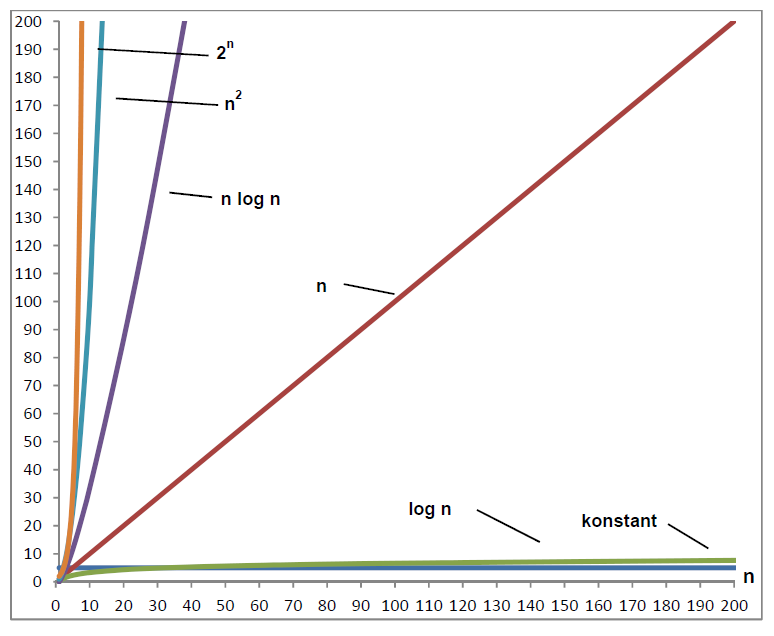
\includegraphics[width=9cm]{images/Algorithmen/Wachstumsfunktionen.png}
\end{minipage}\qquad
\begin{minipage}{10cm}
\textbf{Log-Regeln}\\\\
$log_{10} (a \cdot b) = log_{10}(a)+log_{10}(b)$\\
$log_{10} (\frac{a}{b}) = log_{10}(a) - log_{10}(b)$\\ \\
$log_{10}(a^b) = b \cdot log_{10}(a)$\\
$log_{10}\sqrt[n]{(u)} = \frac{1}{n}\cdot log_{10}(u)$\\ \\
$log_{b}(r) = \frac{log_{a}(r)}{log_{a}(b)}$

\end{minipage}
\subsubsection{Komplexitätsklassen}
Probleme mit ähnlicher Komplexität werden in sogenannten Komplexitätsklassen zusammengefasst. Klassen werden als obere Schranke für den Bedarf einer bestimmten Ressource definiert, in Frage kommen dabei in der Praxis der Zeitbedarf (Zeitkomplexität) und der Speicherbedarf (Platzkomplexität). Auch hier handelt es sich um eine Worst-case-Betrachtung.\\

DTM (Deterministische Turingmaschine): Für jeden Zustand bei gegebenem Input ist der nächste Zustand eindeutig definiert. Ist praktisch realisierbar.\\

\textcolor{red}{N}TM (\textcolor{red}{N}icht deterministische Turingmaschine): Für einen Zustand bei gegebenem Input ist der nächste Zustand \textbf{nicht} eindeutig definiert. Heute noch nicht realisierbar, dient jedoch als Algorithmusausführungsmodell.\\

\begin{minipage}{12cm}
Folgende Klassen sind definiert:\\
\newcommand{\tabitem}{~~\llap{\textbullet}~~}
\begin{tabular}{ll}
\tabitem \textcolor{red}{N}L:                       & Von \textcolor{red}{N}TM auf logarithmischem Platz lösbar \\
\tabitem \textcolor{blue}{P}:                       & Von DTM in \textcolor{blue}{p}olynomialer Zeit lösbar, $O(n^c)$\\
\tabitem \textcolor{red}{N}\textcolor{blue}{P}:     & Von \textcolor{red}{N}TM in \textcolor{blue}{p}olynomialer Zeit lösbar, $O(n^c)$\\
\tabitem \textcolor{blue}{P}SPACE:                  & Von DTM auf \textcolor{blue}{p}olynomialem Platz lösbar\\
\tabitem \textcolor{green}{EXP}TIME:                & Von DTM in \textcolor{green}{exp}onentieller Zeit lösbar, $O(2^n)$\\
\tabitem \textcolor{green}{EXP}SPACE:               & Von DTM auf \textcolor{green}{exp}onentiellem Platz lösbar
\end{tabular}
% \begin{itemize}
% \item \textcolor{red}{N}L: \qquad       Von \textcolor{red}{N}TM auf logarithmischen Platz lösbar
% \item \textcolor{blue}{P}:                        Von DTM in \textcolor{blue}{p}olynomialer Zeit lösbar, $O(n^c)$
% \item \textcolor{red}{N}\textcolor{blue}{P}:       Von NTM in \textcolor{blue}{p}olynomialer Zeit lösbar, $O(n^c)$
% \item \textcolor{blue}{P}SPACE:   Von DTM auf \textcolor{blue}{p}olynomialem Platz lösbar
% \item \textcolor{green}{EXP}TIME:  Von DTM in \textcolor{green}{exp}onentieller Zeit lösbar, $O(2^n)$
% \item \textcolor{green}{EXP}SPACE: Von DTM auf \textcolor{green}{exp}onentiellem Platz lösbar
% \end{itemize}
\end{minipage}~
% \hspace{15cm}
\begin{minipage}{6cm}
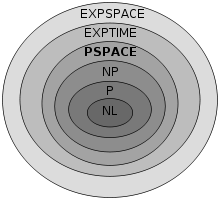
\includegraphics[width=5cm]{images/Algorithmen/KomplexKlassen.png}
\end{minipage}\\

Probleme der Klasse P lassen sich in vernünftiger Zeit lösen. \\
Viele Probleme der Klasse NP lassen sich vermutlich nicht effizient lösen.\\
Bestätigung oder Widerlegung dieses P-NP-Problems ist wohl das wichtigste offene Problem der Informatik.\\
Bekanntes NP-Problem ist das Travelling Salesman Problem (TSP).\\
\\
TSP Lösungsstrategien:
\begin{compactitem}
    \item \textbf{Brute force} alle Varianten durchprobieren
    \item \textbf{Branch and bound} Menge aller Varianten in Teilmengen aufteilen (Branch), mit geeigneten Schranken (Bound) suboptimale Lösungen erkennen und aussortieren
    \item \textbf{Dynamic Programming} Held-Karp Algorithmus
    \item \textbf{Suboptimale Varianten} nicht die optimale Lösung wird angestrebt, sondern nur eine gute
\end{compactitem}

\subsection{Suchalgorithmen}
\subsubsection{Listensuche}
Finde Wert in einer Liste.\\

\textbf{Listendefinition}
\lstinputlisting[language=C++]{code/Listendefinition.cpp}
\ \newline
\textbf{Vereinfachte Listendefinition}
\begin{multicols}{2}
\lstinputlisting[language=C++]{code/VereinfachteListendefinition.cpp}
\vfill\null
\columnbreak
Mit dieser vereinfachten Listendefinition können wir uns auf die Algorithmen konzentrieren, da die Komplexität einer (verketteten) Liste wegfällt. Die Algorithmen können 1:1 auf eine kompliziertere Listenstruktur übertragen werden.
\end{multicols}
\ \newline
\textbf{Variante 1: Lineare Suche}\\
Die einfachste Suchmethode ist, von vorne nach hinten Element um Element zu überprüfen bis das gesuchte Element gefunden oder das Listenende erreicht ist. Wenn nicht bekannt ist, ob die Liste irgendwie sortiert ist, ist das die einzige mögliche Suchmethode. \\
Komplexität: O(n)
\lstinputlisting[language=C++]{code/LineareSuche.cpp}
\ \newline
\textbf{Variante 2: Lineare Suche mit Sentinel}\\
Die einzige Methode, den obigen Algorithmus zu beschleunigen, besteht in der Vereinfachung der
Schleifenbedingung. Bei der linearen Suche mit Sentinel (Wächter) wird einfach am Ende der Liste ein Hilfselement eingefügt, das auf den Wert des gesuchten Elementes gesetzt wird. Der Algorithmus terminiert so auch ohne die Abfrage der Listenlänge, allerdings wird ein Platz in der Liste für den Sentinel geopfert.\\
Die Schleife wird etwas schneller durchlaufen, aber die Komplexität ist noch immer O(n).
\lstinputlisting[language=C++]{code/LineareSucheMitSentinel.cpp}
\ \newline
\textbf{Variante 3: Binäre Suche}\\
Diese Suche funktioniert nur, wenn die Liste der Reihe nach sortiert ist.\\
Man geht von der Mitte der Liste aus, ist der gegebene Wert grösser als die Mitte sucht man in der oberen Hälfte auf dieselbe Art weiter, ansonsten in der unteren Hälfte.\\
Liegt der Wert am Rande ist die Suche auf diese Art erfolglos.\\
Komplexität: O(log(n))\\
\lstinputlisting[language=C++]{code/BinaereSuche.cpp}
Beispiel "'Suche 53"':\\
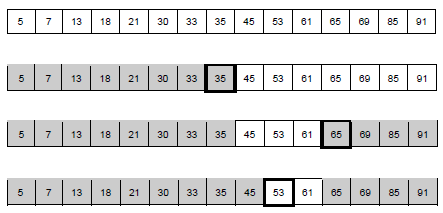
\includegraphics[width=0.4\textwidth]{images/Algorithmen/BinaereSuche.png}

\subsubsection{Mustersuche}
Bei der Mustersuche (string search) geht es darum, ein ganzes Stringmuster (Pattern) in einem vorgegebenen Text zu suchen. Wenn nur ein einzelnes Zeichen gesucht werden müsste, wäre dies identisch mit der Listensuche. Bei der Suche eines ganzen Patterns wird der Algorithmus aber bedeutend komplexer. Da die Mustersuche eine fundamentale Operation in jeder Textverarbeitung ist, besteht hier ein grosses Interesse, einen möglichst effizienten Algorithmus zu finden.\\

\textbf{Variante Naiver Algorithmus}\\
Der naive Algorithmus ist sehr einfach, es wird einfach Buchstabe um Buchstabe verglichen, bis eine Diskrepanz eintritt. Anschliessend wird das Pattern um eine Position weitergeschoben und wieder
Buchstabe um Buchstabe verglichen. Wenn die Diskrepanz schon bei einem der ersten Buchstaben auftritt, ist die Performance des Algorithmus OK. Wenn jedoch viele Buchstaben übereinstimmen bis endlich eine Diskrepanz auftritt, dann ist die Performance sehr schlecht. Im schlechtesten Fall ist der Algorithmus O(n·m), wobei n die Länge des Textes und m die Länge des Patterns ist.
\lstinputlisting[language=C++]{code/NaiverAlgorithmus.cpp}
Bei effizienteren Suchalgorithmen (z.B. KMP-Algorithmus oder BM-Algorithmus) wird bei einer Nichtübereinstimmung nicht nur um ein Zeichen sondern um eine möglichst hohe Anzahl Zeichen geschoben. Die Intelligenz liegt hier beim Herausfinden dieser Anzahl. Dazu bedarf es Informationen, die vom Pattern abhängig sind. Dies wird in einer sogenannten Präfixanalyse vor der eigentlichen Suche durchgeführt.


\subsection{Sortieralgorithmen}

\subsubsection{Interne vs. externe Sortierverfahren}
\begin{itemize}
    \item Bei den \textbf{internen Sortierverfahren} besteht auf sämtliche Daten ein wahlfreier Zugriff (random access). Die Daten liegen vollständig im Hauptspeicher vor. Die internen Sortierverfahren werden auch als Verfahren zum Sortieren von Feldern (Arrays) bezeichnet.
    \item Bei den \textbf{externen Sortierverfahren} kann nur sequentiell auf die Daten zugegriffen werden. Die Daten sind in Files auf langsameren externen Massenspeichern wie z.B. Magnetbändern oder Harddisks gespeichert. Die externen Sortierverfahren werden auch als Verfahren zum Sortieren von Files bezeichnet.
\end{itemize}

\subsubsection{Forderungen an interne Sortierverfahren}
\begin{itemize}
    \item \textbf{Speicher:} Sämtliche Daten liegen im Hauptspeicher. Nebst den vorhandenen Daten ist nur eine \textbf{feste Anzahl von (Hilfs-) Variablen} erlaubt (In-place Algorithmen).
    \item \textbf{Effizienz:} Nur Vergleiche (Comparison) und Zuweisungen (Move) werden betrachtet.
    (Bei den Zuweisungen werden nur die Zuweisungen der zu sortierenden Daten berücksichtigt. Zuweisungen von Indizes werden vernachlässigt, da sie in der Regel wesentlich schneller ablaufen, da sie sicher in Registern liegen. Auch die Vergleiche der Indizes werden vernachlässigt.)
    \item \textbf{Stabilität:} Ein Sortierverfahren ist dann stabil, wenn es die relative Reihenfolge gleicher Schlüssel beibehält. (Beispielsweise soll eine alphabetisch geordnete Liste von Wettkämpfern, die nach den Wettkampfnoten sortiert wird, die alphabetische Reihenfolge der Wettkämpfer bei gleichen Noten beibehalten.)
\end{itemize}

\subsubsection{Einfache interne Sortierverfahren}
\begin{itemize}
    \item Gut verständlich
    \item Meist stabil
    \item Komplexität $O(n^2)$
\end{itemize}
\textbf{Variante 1: Direktes Aussuchen (Straight selection)}\\
Beim direkten Aussuchen wird der noch unsortierte Teil nach seinem kleinsten Element durchsucht. Dieses wird dann mit dem ersten Element im unsortierten Teil vertauscht.\\
Komplexität der Vergleiche: $O(n^2)$\\
Komplexität der Zuweisungen: $O(n)$\\
\begin{multicols}{2}
\lstinputlisting[language=C++]{code/DirektesAussuchen.cpp}
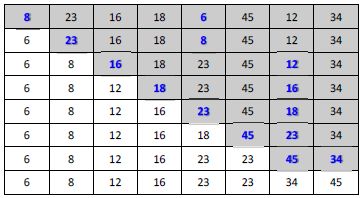
\includegraphics[width=0.5\textwidth]{images/Algorithmen/DirektesAussuchen.png}
\end{multicols}
\ \newline
\textbf{Variante 2: Direktes Einfügen (Straight insertion)}\\
Das erste Element des unsortierten Teiles wird im sortierten Teil direkt an der richtigen Stelle entsprechend seiner Grösse eingefügt. Alle grösseren bereits sortierten Elemente müssen verschoben werden.\\
Komplexität der Vergleiche: $O(n^2)$\\
Komplexität der Zuweisungen: $O(n^2)$\\
Effizient, wenn die Daten schon möglichst sortiert sind. Der schlechteste Fall tritt dann ein, wenn die Daten zu Beginn absteigend sortiert sind.
\begin{multicols}{2}
\lstinputlisting[language=C++]{code/DirektesEinfuegen.cpp}
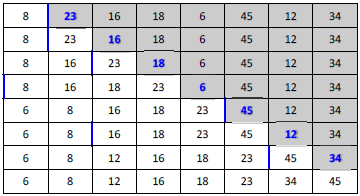
\includegraphics[width=0.5\textwidth]{images/Algorithmen/DirektesEinfuegen.png}
\end{multicols}
\ \newline
\textbf{Variante 3: Bubblesort}\\
Jeweils benachbarte Elemente werden vertauscht, wenn sie nicht wie gewünscht geordnet sind. Bei jedem Durchlauf steigt dabei das relativ grösste Element wie eine Blase (bubble) im Wasser auf.\\
Komplexität der Vergleiche: $O(n^2)$\\
Komplexität der Zuweisungen: $O(n^2)$\\
\begin{multicols}{2}
\lstinputlisting[language=C++]{code/Bubblesort.cpp}
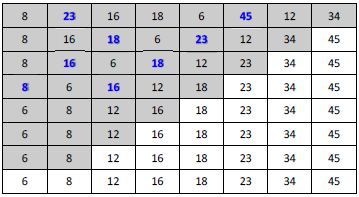
\includegraphics[width=0.5\textwidth]{images/Algorithmen/Bubblesort.png}
\end{multicols}

\subsubsection{Schnelle interne Sortierverfahren}
\begin{itemize}
    \item Schwerer verständlich als einfache Sortierverfahren
    \item Instabil
    \item Komplexität $O(n\cdot log(n))$
\end{itemize}
\textbf{Variante 1: Quicksort}\\
Je grösser die Distanz beim Austauschen von Elementen ist, umso effizienter ist der Algorithmus. Dies nutzt Quicksort aus.\\\\
Formale Beschreibung:
\begin{enumerate}
\item Wähle einen beliebigen Pivotwert aus dem Array aus.
\item Laufe von linker Arraygrenze so lange nach innen, bis ein \textbf{nicht kleineres}
Element als der Pivotwert gefunden wird.
\item Laufe von rechter Arraygrenze so lange nach innen, bis ein \textbf{nicht grösseres} Element gefunden wird.
\item Vertausche die beiden Elemente.
\item Wiederhole Schritt 2-4 so lange, bis sich die beiden Indizes getroffen haben.
\item Das nun entstandene Teilfeld links besteht nur aus Elementen, die kleiner oder gleich dem Pivotwert sind, das Teilfeld rechts besteht nur aus Elementen, die grösser oder gleich dem Pivotwert sind.
\item Sortiere diese beiden Teilfelder wiederum (rekursiv), bis nur noch Teilfelder mit einem einzigen Element übrig bleiben.
\end{enumerate}
\begin{multicols}{2}
\lstinputlisting[language=C++]{code/Quicksort.cpp}
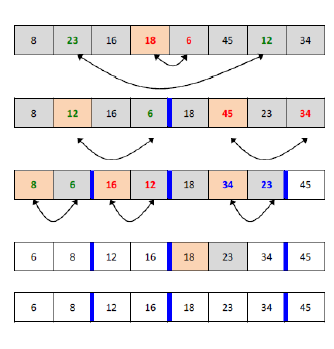
\includegraphics[width=0.5\textwidth]{images/Algorithmen/Quicksort.png} \ \\ \ \\
\end{multicols}
Bester Fall: Wenn als Pivot jedes mal der Median des Feldes getroffen wird $\rightarrow O(n\cdot log(n))$\\
Schlechtester Fall: Wenn jedes Mal das Minimum oder Maximum getroffen wird $\rightarrow O(n^2))$\\\\
Schnell, weil das Austauschen von unsortierten Elementen über möglichst grosse Distanzen erfolgt.\\\\
\textbf{Median}: Der Median einer Anzahl von Werten ist die Zahl, welche an der mittleren Stelle steht, wenn man die Werte nach Größe sortiert. Bsp: {4, 1, 37, 2, 1} Median = 2\\\\
Eine vernünftige Wahl des Pivots ist also wichtig. Ein Ansatz ist die median-of-3 Strategie, bei welcher der Median aus dem ersten, letzten und mittleren Element eines Bereiches gebildet und als Pivot verwendet wird. Bei bösartig zusammengestellten Listen (median-of-3-killers) kann dies jedoch zu Problemen führen.\\
\ \newline
\textbf{Variante 2: Introsort}
\begin{itemize}
    \item Ist in jedem Fall $O(n\cdot log(n))$
    \item Setzt bei den Schwächen von Quicksort an $\rightarrow$ startet mit Quicksort und wechselt automatisch auf Heapsort (ein weiterer Algorithmus), wenn die Rekursionstiefe einen definierten Wert überschreitet.
\end{itemize}
\subsubsection{Anzahl der Vergleiche (Compare) bei Sortieralgorithmen}
\begin{tabular}{|c|c|c|c|c|}
\hline
Algorithmus & $C_{min}$ & $C_{ave}$ & $C_{max}$ & $O_C(\cdot)$ \\
\hline
Straight Selection & \multicolumn{3}{c|}{$\frac{n}{2}\cdot (n-1)$} & $n^2$ \\
\hline
Straight Insertion & $n-1$ & $\frac{1}{4}\cdot (n^2 + 3n -4)$ & $\frac{1}{2}\cdot (n^2+n-2)$ & $n^2$ \\
\hline
Bubblesort & \multicolumn{3}{c|}{$\frac{n}{2}\cdot (n-1)$} & $n^2$ \\
\hline
Quicksort & $n\cdot log_{2}(n)$ & $2\cdot n \cdot ln(n)$ & $\frac{1}{2}\cdot (n+3)(n+2)-10$ & $n^2$ \\
\hline
\end{tabular}

\subsubsection{Anzahl der Zuweisungen (Move) bei Sortieralgorithmen}
\begin{tabular}{|c|c|c|c|c|}
\hline
Algorithmus & $M_{min}$ & $M_{ave}$ & $M_{max}$ & $O_M(\cdot)$ \\
\hline
Straight Selection & \multicolumn{3}{c|}{$3\cdot (n-1)$} & $n$ \\ % & $3\cdot (n-1)$ & $3\cdot (n-1)$ & $n$ \\
\hline
Straight Insertion & $3\cdot (n-1)$ & $\frac{1}{4}\cdot (n^2 + 11n -12)$ & $\frac{1}{2}\cdot (n^2+5n-6)$ & $n^2$ \\
\hline
Bubblesort & $0$ & $\frac{3}{4}\cdot n\cdot (n-1)$ & $\frac{3}{2}\cdot n\cdot (n-1)$ & $n^2$ \\
\hline
Quicksort & $0$ & $n\cdot ln(n)$ & $\frac{3}{4}\cdot n\cdot log_{2}(n)$ & $n\cdot log_{10}(n)$ \\
\hline
\end{tabular}

\subsection{Kombination von Suchen und Sortieren}
Eine Liste wird nie zum Selbstzweck sortiert, sondern nur wenn auch gesucht werden muss. Bei einer sich nicht ändernden Liste kann binär gesucht werden. Bei häufig ändernden Daten, die auch gesucht werden müssen, bieten sich binäre Suchbäume als Datenstruktur an (siehe Literatur).


\subsection{Systemfunktionen für Suchen und Sortieren}

\subsubsection{In C}
\begin{tabular}{|llll|}
\hline
\textbf{Funktion} & \textbf{Bibliothek} & \textbf{Algorithmus} & \textbf{Bemerkungen} \\
\hline
bsearch() & \textless stdlib.h\textgreater & Binäre Suche in Arrays & \\
\hline
qsort() & \textless stdlib.h\textgreater & Quicksort & instabil \\
\hline
\end{tabular}

\subsubsection{In C++}
\begin{tabular}{|llll|}
\hline
\textbf{Funktion} & \textbf{Bibliothek} & \textbf{Algorithmus} & \textbf{Bemerkungen} \\
\hline
binary\_search() & \textless algorithm\textgreater & Binäre Suche & \\
\hline
sort() & \textless algorithm\textgreater & Introsort & instabil \\
\hline
stable\_sort() & \textless algorithm\textgreater & Mergesort & stabil \\
\hline
\end{tabular}
